\documentclass[10pt,aspectratio=169,serif]{beamer}

\usepackage[fontset=none, scheme=plain]{ctex}
\IfFontExistsTF{Songti SC}{%
	\setCJKmainfont{Songti SC}[AutoFakeSlant=0.2]%
	\setCJKsansfont{Songti SC}[AutoFakeSlant=0.2]%
}{%
	\setCJKmainfont{FandolSong-Regular}[Extension=.otf,BoldFont=FandolSong-Bold,AutoFakeSlant=0.2]%
	\setCJKsansfont{FandolSong-Regular}[Extension=.otf,BoldFont=FandolSong-Bold]%
}
\usepackage{amsmath,amssymb,graphicx,tikz,booktabs,multicol,calligra}
\usepackage{pgfplots}
\pgfplotsset{compat=1.18}
\usepackage{tcolorbox}
\tcbuselibrary{skins}
\usepackage{XyygU}
\usepackage{caption}
\captionsetup[figure]{name=图,labelsep=period}

\usetikzlibrary{arrows.meta,positioning,calc}

% 公式间距
\setlength{\abovedisplayskip}{0pt plus 2pt minus 2pt}
\setlength{\belowdisplayskip}{0pt plus 2pt minus 2pt}

\title[充分条件与必要条件练习]{1.4 充分条件与必要条件（练习）}
\subtitle{充分条件、必要条件与充要条件}
\author{}
\institute{}
\date{2026-10-16}

\begin{document}

\begin{frame}
  \titlepage
\end{frame}

% ========== 第一部分：充分条件与必要条件（P20练习） ==========
\begin{frame}[t]{核心概念回顾}
\begin{tcolorbox}[colback=blue!5,colframe=blue,title=\textbf{充分条件、必要条件、充要条件}]
若 $p \Rightarrow q$，则称 $p$ 是 $q$ 的\alert{充分条件}，$q$ 是 $p$ 的\alert{必要条件}。\\[0.5em]
若 $p \Leftrightarrow q$（即 $p\Rightarrow q$ 且 $q\Rightarrow p$），则称 $p$ 是 $q$ 的\alert{充要条件}。
\end{tcolorbox}
\end{frame}

% ===== 练习1 =====
\begin{frame}[t]{练习1：判断充分条件}
\textbf{1.} 下列"若 $p$，则 $q$"形式的命题中，哪些命题中的 $p$ 是 $q$ 的充分条件？\\
(1) 若平面内点 $P$ 在线段 $AB$ 的垂直平分线上，则 $PA=PB$；\\
(2) 若两个三角形的两边及一边所对的角分别相等，则这两个三角形全等；\\
(3) 若两个三角形相似，则这两个三角形的面积比等于周长比的平方。
\end{frame}

\begin{frame}[t]{练习1 解答}
\begin{tcolorbox}[colback=orange!10,colframe=orange,title=\textbf{解}]
\textbf{(1) 是}。由线段垂直平分线的性质定理：垂直平分线上的点到线段两端距离相等，故 $p\Rightarrow q$。

\textbf{(2) 不是}。"两边及一边对角相等"即 SSA，不能判定三角形全等（可能一个是锐角三角形、一个是钝角三角形），故 $p\nRightarrow q$。

\textbf{(3) 是}。相似三角形面积比等于相似比的平方，而周长比等于相似比，故面积比 =（周长比）$^2$，即 $p\Rightarrow q$。

\vspace{0.5em}
\small（结论：(1)(3) 中的 $p$ 是 $q$ 的充分条件）
\end{tcolorbox}
\end{frame}

% ===== 练习2 =====
\begin{frame}[t]{练习2：判断必要条件}
\textbf{2.} 下列"若 $p$，则 $q$"形式的命题中，哪些命题中的 $q$ 是 $p$ 的必要条件？\\
(1) 若直线 $l$ 与 $\odot O$ 有且仅有一个交点，则 $l$ 为 $\odot O$ 的一条切线；\\
(2) 若 $x$ 是无理数，则 $x^2$ 也是无理数。
\end{frame}

\begin{frame}[t]{练习2 解答}
\begin{tcolorbox}[colback=orange!10,colframe=orange,title=\textbf{解}]
$q$ 是 $p$ 的必要条件 $\Longleftrightarrow$ $p\Rightarrow q$。

\textbf{(1) 是}。由切线的定义：直线与圆有且只有一个公共点时，该直线就是圆的切线，故 $p\Rightarrow q$。

\textbf{(2) 不是}。反例：$x=\sqrt{2}$ 是无理数，但 $x^2=2$ 是有理数，故 $p\nRightarrow q$。

\vspace{0.5em}
\small（结论：(1) 中的 $q$ 是 $p$ 的必要条件）
\end{tcolorbox}
\end{frame}

% ===== 练习3 =====
\begin{frame}[t]{练习3：平行线的充分与必要条件}
\textbf{3.} 如图，直线 $a$ 与 $b$ 被直线 $l$ 所截，分别得到了 $\angle 1$，$\angle 2$，$\angle 3$ 和 $\angle 4$。请根据这些信息，写出几个"$a \parallel b$"的充分条件和必要条件。

\vspace{0.5em}
\begin{center}
\begin{tikzpicture}[scale=1.2]
% 直线a
\draw[thick] (-3,1) -- (3,1);
\node[left] at (-3,1) {$a$};
% 直线b
\draw[thick] (-3,-1) -- (3,-1);
\node[left] at (-3,-1) {$b$};
% 截线l
\draw[thick] (-1.5,2) -- (0.5,-2);
\node[above right] at (-1.5,2) {$l$};
% 角标注（在a与l交点）
\node at (-1.3,1.3) {$4$};
\node at (-0.9,1.3) {$3$};
\node at (-0.9,0.7) {$2$};
% 在b与l交点
\node at (0.2,-0.7) {$1$};
\end{tikzpicture}
\end{center}
\end{frame}

\begin{frame}[t]{练习3 解答}
\begin{tcolorbox}[colback=orange!10,colframe=orange,title=\textbf{解}]
\textbf{"$a\parallel b$"的充分条件}（即由该条件可推出 $a\parallel b$）：
\begin{itemize}
  \item $\angle 1 = \angle 2$（同位角相等）；
  \item $\angle 2 = \angle 3$（内错角相等）；
  \item $\angle 3 + \angle 4 = 180^\circ$（同旁内角互补）。
\end{itemize}

\vspace{0.5em}
\textbf{"$a\parallel b$"的必要条件}（即由 $a\parallel b$ 可推出该条件）：
\begin{itemize}
  \item $\angle 1 = \angle 2$；
  \item $\angle 2 = \angle 3$；
  \item $\angle 3 + \angle 4 = 180^\circ$。
\end{itemize}
\vspace{0.5em}
\small（在平行线判定与性质中，上述三组条件互为充要条件，因此既是充分又是必要）
\end{tcolorbox}
\end{frame}

% ========== 第二部分：充要条件（P22练习） ==========
\begin{frame}[t]{第二部分：充要条件（教材第22页练习）}
\end{frame}

% ===== 练习4 =====
\begin{frame}[t]{练习4：判断充要条件}
\textbf{1.}（充要条件练习第1题）下列各题中，哪些 $p$ 是 $q$ 的充要条件？\\
(1) $p$：三角形为等腰三角形，$q$：三角形存在两角相等；\\
(2) $p$：$\odot O$ 内两条弦相等，$q$：$\odot O$ 内两条弦所对的圆周角相等；\\
(3) $p$：$A \cap B$ 为空集，$q$：$A$ 与 $B$ 之一为空集。
\end{frame}

\begin{frame}[t]{练习4 解答}
\begin{tcolorbox}[colback=orange!10,colframe=orange,title=\textbf{解}]
\textbf{(1) 是}。等腰三角形两底角相等；反之，有两角相等的三角形是等腰三角形（等角对等边）。故 $p\Leftrightarrow q$。

\textbf{(2) 不是}。同圆中两条弦相等，则它们所对的圆心角相等，所对的圆周角\alert{相等或互补}（一条弦所对的圆周角有两个，分别在弦两侧，和为 $180^\circ$）。故 $p\nRightarrow q$（当两弦所对圆周角取互补时不相等）。

\textbf{(3) 不是}。反例：$A=\{1\}, B=\{2\}$，$A\cap B=\varnothing$ 但 $A,B$ 都非空。故 $p\nRightarrow q$。

\vspace{0.5em}
\small（结论：只有 (1) 中 $p$ 是 $q$ 的充要条件）
\end{tcolorbox}
\end{frame}

% ===== 练习5 =====
\begin{frame}[t]{练习5：写出全等与相似的充要条件}
\textbf{2.}（充要条件练习第2题）分别写出"两个三角形全等"和"两个三角形相似"的几个充要条件。
\end{frame}

\begin{frame}[t]{练习5 解答}
\begin{tcolorbox}[colback=orange!10,colframe=orange,title=\textbf{解}]
\textbf{两个三角形全等的充要条件：}
\begin{itemize}
  \item 三边对应相等（SSS）；
  \item 两边及其夹角对应相等（SAS）；
  \item 两角及其夹边对应相等（ASA）；
  \item 两角及其中一角的对边对应相等（AAS）；
  \item 斜边和一条直角边对应相等（HL，直角三角形）。
\end{itemize}

\textbf{两个三角形相似的充要条件：}
\begin{itemize}
  \item 两角分别相等；
  \item 三边成比例；
  \item 两边成比例且夹角相等。
\end{itemize}
\end{tcolorbox}
\end{frame}

% ===== 练习6 =====
\begin{frame}[t]{练习6：证明等腰梯形的充要条件}
\textbf{3.}（充要条件练习第3题）证明：如图，梯形 $ABCD$ 为等腰梯形的充要条件为 $AC=BD$。

\vspace{0.5em}
\begin{center}
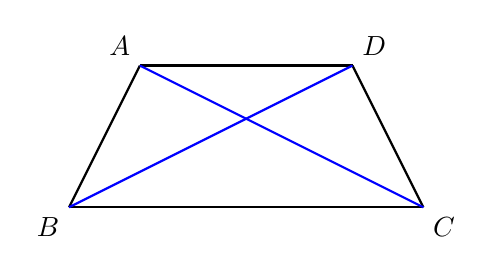
\begin{tikzpicture}[scale=0.9]
% 梯形ABCD，AD∥BC
\draw[thick] (-1.5,1) -- (1.5,1);
\node[above left] at (-1.5,1) {$A$};
\node[above right] at (1.5,1) {$D$};
\draw[thick] (-2.5,-1) -- (2.5,-1);
\node[below left] at (-2.5,-1) {$B$};
\node[below right] at (2.5,-1) {$C$};
\draw[thick] (-1.5,1) -- (-2.5,-1);
\draw[thick] (1.5,1) -- (2.5,-1);
% 对角线
\draw[thick,blue] (-1.5,1) -- (2.5,-1);
\draw[thick,blue] (1.5,1) -- (-2.5,-1);
\end{tikzpicture}
\end{center}
\end{frame}

\begin{frame}[t]{练习6 解答}
\begin{tcolorbox}[colback=orange!10,colframe=orange,title=\textbf{证明：充分性与必要性}]
设梯形 $ABCD$ 中 $AD\parallel BC$。

\textbf{必要性（$\Rightarrow$）：} 若 $ABCD$ 为等腰梯形，则两腰 $AB=CD$。在 $\triangle ABC$ 和 $\triangle DCB$ 中：$AB=DC$，$\angle ABC=\angle DCB$（等腰梯形底角相等），$BC$ 公共边，故 $\triangle ABC\cong\triangle DCB$（SAS），从而 $AC=BD$。

\textbf{充分性（$\Leftarrow$）：} 若 $AC=BD$，过 $D$ 作 $DE\parallel AC$ 交 $BC$ 延长线于 $E$，则 $ACED$ 为平行四边形，故 $DE=AC=BD$，$\triangle DBE$ 为等腰三角形，$\angle E=\angle DBE$。又 $\angle ACB=\angle E$，故 $\angle ACB=\angle DBC$。在 $\triangle ABC$ 和 $\triangle DCB$ 中：$AC=DB$，$\angle ACB=\angle DBC$，$BC$ 公共边，故 $\triangle ABC\cong\triangle DCB$，得 $AB=DC$，即梯形 $ABCD$ 为等腰梯形。

\vspace{0.3em}
\small（综上，梯形 $ABCD$ 为等腰梯形 $\Longleftrightarrow$ $AC=BD$）
\end{tcolorbox}
\end{frame}

\begin{frame}[c]
  \begin{center}
    {\Huge\calligra Thanks!}
  \end{center}
\end{frame}

\end{document}
